\section{Support Vector Machines}
Perceptron is instable: It does not choose the best classifier, but just any.

\subsection{Maximum Margin Classifiers}
\textbf{Maximum-margin criterion: } Maximize the margin between the classes.

\begin{equation*}
	\begin{gathered}
		\min_{\mathbf w, w0}\frac{1}{2}\norm{\mathbf w}^2 \\
		\textit{s.t.}: 1 - y_i(\mathbf w^Tx_i + w_0) \leq 0
	\end{gathered}
\end{equation*}

\subsection{Constrained Convec Optimization using Lagrange}
\subsubsection{Lagrange}
Solve
$\min_w f(w)$ s.t. $ g_i(w) = 0$ by solving

$$
	\mathcal L(w, \beta) = f(w) + \sumi l \alpha_i g_i(w)
$$
where $\alpha_i$ are called lagrangian multipliers.

\subsubsection{Lagrange Dual Formulation}
$\min_w f(w) \textit{ s.t. } g_i(w) = 0, h_j(w) \leq 0$\\
\begin{enumerate}
  \item  Generalized Lagrangian: $\mathcal L(\mathbf w, \lambda, \alpha) = f(\mathbf w) + \sum_i\lambda_ig_i(\mathbf w) + \sum_{j} \alpha_jh_j(\mathbf w), \alpha_j\geq 0$ \
  \item  
  $$
d^*=\max_{\lambda, \alpha: \alpha_j \geq 0}\min_\textbf{w}\mathcal{L}(\mathbf{w}, \lambda, \alpha) \leq \min_\textbf{w}\max_{\lambda, \alpha: \alpha_j \geq 0} \mathcal{L}(\mathbf{w}, \lambda, \alpha) = p^*
$$
\textbf{Strong Duality: } $d^* = p^*$. \\
\textbf{Slaters Conditions: } is there a \textbf{w} such that $g_i(\textbf{w}) = 0$ and $h_j(\textbf{w}) < 0$? Sufficient for Strong duality
  \item solve dual $\max_{\alpha, \lambda} \min_w  \mathcal L$, get $\alpha_i$
  \item compute $\alpha_i$ to compute the weights. This way, we don't have to compute the scalar product $\transp{w}x $, which may be expensive if $d$ is large.
\end{enumerate}

$\alpha_i = 0$ for all but a few vectors (the support vectors). We can then compute: 
\sepline

\subsubsection{Lecture: } 
$$
	\min_w f(w)\quad \textit{ s.t. } g_i(w) = 0, h_j(w) \leq 0
$$ \textit{\textbf{("primal optimization problem")}}
\begin{enumerate}
	\item Solve using generalized Lagrangian: 
	$$\mathcal L(\mathbf w, \lambda, \alpha) = f(\mathbf w) + \sum_i\lambda_ig_i(\mathbf w) + \sum_{j} \alpha_jh_j(\mathbf w), \alpha_j\geq 0
	$$
	$\lambda_i, \alpha_i$ are the lagrangian multipliers.
	\item Check\textbf{ Slaters condition:} \textit{Is there $w$ s.t. $g_i(w) = 0$ and $h_j(w) < 0$ for $i\leq n, j\leq m$} (conditions strictly fullfilled). \\
	If $\w$ violates the constraints, we can verify that $\max \mathcal L = \infty$. Otherwise, $\max \mathcal L = f(\w)$.
	
	We can hence consider 
	$$
		\min_w \max_{\alpha, \lambda} \mathcal L(\w, \lambda, \alpha)
	$$
	
	We have
	$$
		\underbrace{\max_{\alpha, \lambda} \min_w  \mathcal L(\w, \lambda, \alpha)}_{\textit{Dual Formulation}}\leq \min_w \max_{\alpha, \lambda} \mathcal L(\w, \lambda, \alpha)
	$$
	\item Solve
	\begin{equation*}
		\begin{gathered}
			\frac{\partial\mathcal L}{\partial \mathbf w} = 0,
			g_i(\mathbf w) = 0, g_j(\mathbf w) \leq 0 \\
			\alpha_j \geq 0
			\alpha_jh_j(\mathbf w) = 0 \\
			\textit{(compl. slackness)}
		\end{gathered}
	\end{equation*}
\end{enumerate}

\subsubsection{Strong duality}
\begin{itemize}
 	\item Strong duality: primal optimal objective and the dual optimal objective are equal.  \\
	 $\max_{\lambda, \alpha} \min_w \mathcal L(w, \lambda, \alpha) = \min_w f(w)$
	 \item Slater's condition is a suffcient condition for strong duality.

	\item Weak duality
	 $\max_{\lambda, \alpha} \min_w \mathcal L(w, \lambda, \alpha) \leq \min_w f(w)$
\end{itemize}

\subsection{SVM: Compute a maximum margin classifier}
Assume the 2 classes are linearly separable.
\begin{center}
	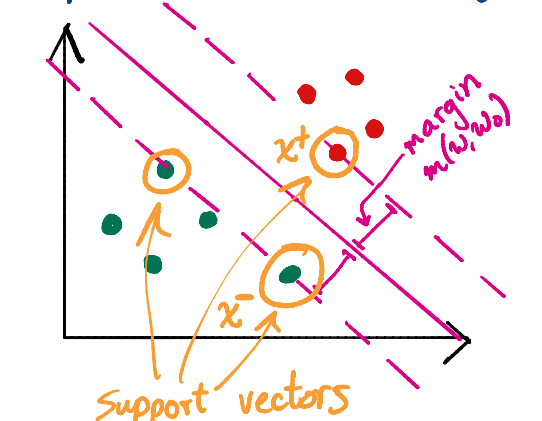
\includegraphics[width=0.6\columnwidth]{images/7-SVM-max-margin}
\end{center}

\textbf{Goal: }
\begin{equation*}
	\begin{gathered}
		\max_{\w, w_0} 2m(\w,w_0) \quad\textit{s.t.} \\
		\w^Tx_i + w_0 > 0 \iff y_i = +1 \\
		\w^Tx_i + w_0 < 0 \iff y_i = -1 \\
		\equiv y_i(\w^Tx_i + w_0) \geq b > 0
	\end{gathered}
\end{equation*}

\begin{align*}
	2m(\w, w_0) &= \norm{\textit{proj}_\w x^+ - \textit{proj}_\w x^-} \\
				&= \norm{\frac{\w^T x^+}{\norm{\w}^2} \w -\frac{\w^T x^-}{\norm{\w}^2} \w} \\
				&= \frac{1}{\norm{\w}} |\w^T x^+ - \w^T x^-|
\end{align*}

$m(\w, w_0)$ does not depend on $\norm{\w}$ nor $w_0$: Let $\gamma \in \R: $

$$
	m(\gamma \w, w_0) = \frac{1}{\gamma\norm{\w}} |\gamma\w^Tx^+ - \gamma\w^Tx^-| = m(\w, w_0)
$$

There is $w^*, w_0^*$ optimal such that $w^{*T}x^+ + w_o^* = 1$ and $w^{*T}x^- + w_0^* = -1$:

\begin{align*}
	2m(\w^*, w_0^*) &= \frac{1}{\norm{\w^*}} |\w^{*T}x^+ - \w^{*T} x^-| = \frac{2}{\norm{\w^*}}\\
	w^{*T}x_i + w_0^* &\geq w^{*T}x^+ + w_0^* = 1 \textit{ if } y_i = +1 \\
	w^{*T}x_i + w_0^* &\leq w^{*T}x^- + w_0^* = 1 \textit{ if } y_i = -1 \\
\end{align*}

\textbf{SVM formulation: } 
\begin{equation*}
	\begin{gathered}
		\min_{\mathbf w, w0}\frac{1}{2}\norm{\mathbf w}^2 \\
		\textit{s.t.}:  y_i(\mathbf w^T x_i + w_0) \geq 1
	\end{gathered}
\end{equation*}

\textbf{Slaters Condition}
\begin{itemize}
	\item By linear separation: $\exists \w, w_0: y_i(\w^T x_i + w_0)\geq 1, i\leq n$
	\item Take $\gamma>1 \implies (\gamma\w, \gamma w_0)$
	\begin{align*}
		y_i(\gamma\w^T x_i + \gamma w_0) &= \gamma y_i(\w^T x_i + w_0) \\
										&> y_i(\w^T x_i + w_0 \\
										&\geq 1
	\end{align*}
\end{itemize}


\textbf{Dual}
\begin{align*}
	\mathcal L(\w, w_0, \alpha) &= \frac{1}{2}\norm{w}^2 + \sum_i\alpha_i(1. yi(\w^Tx_i + w_0)), \alpha_i \geq 0 \\
	&= \frac{1}{2}\w^T\w + \sum_i\alpha_i \\
	&\quad\quad\quad- \sum_i\alpha_i y_i\w^Tx_i - \sum_i\alpha_i y_i w_0 \\
	\frac{\partial\mathcal L}{\partial \w} &= \w + 0- \sum_i\alpha_i y_i x_i + 0 \\
	\frac{\partial\mathcal L}{\partial w_0} &= 0 + 0 + 0 - \sum_i\alpha_i y_i
\end{align*}

Setting the derivatives to $0$ yields:
\begin{equation*}
	w^* = \sum_i\alpha_i y_i x_i, \quad \sum_i \alpha_i y_i = 0 
\end{equation*}
Plugging this into the dual formulation, we get:

\begin{equation*}
	\begin{gathered}
		\max_\alpha \frac{1}{2}\sum_{i,j} \alpha_i\alpha_jy_iy_jx_i^Tx_j + \sum_i \alpha_i - \sum_{i,j} \alpha_i\alpha_jy_iy_jx_i^Tx_j \\
		\alpha_i\geq 0, \sum_i\alpha_i y_i = 0
	\end{gathered}
\end{equation*}

which simplifies to
\begin{equation*}
	\begin{gathered}
		\max_\alpha \sum_i \alpha_i-\frac{1}{2}\sum_{i,j} \alpha_i\alpha_jy_iy_jx_i^Tx_j\\
		\alpha_i\geq 0, \sum_i\alpha_i y_i = 0
	\end{gathered}
\end{equation*}

\subsection{Shockfish}
Shockfish aims at predicting parking lot occupancy. Classification task: Occupied vs. non-occupied?

\textbf{Idea:}
\begin{itemize}
	\item Sense earth magnetic fields and measure deviations
	\item Deviations occur when a large mass (e.g. truck) is close to the sensor
	\item Sensor at each parking lot, use readings to detect presence of vehicle.
\end{itemize}

\textbf{Sensor Readings: }
\begin{itemize}
	\item Center Values: Temperature and other physical variations
	\item Data set: $\textit{signal}(t) = \textit{reading}(t) - \textit{center}(t)$
\end{itemize}

\textbf{Problem: }Truck also influences sensor measurements of neighboring sensors
\begin{itemize}
	\item[$\Rightarrow$] Weak coupling of neighboring sensors 
\end{itemize}

\subsubsection{Challenges}
\begin{itemize}
	\item Design new algorithm
	\item Label the readings of three weeks based on camera imagery
	\item find approp. data preprocessing filters
	\item Performance measures: Accuracy, Generalization (over sensors and parking lots).
	\item Have to carefully specify conditioning on sensor or parking lot.
\end{itemize}

\subsubsection{Problems in Real World Applications}
\begin{itemize}
	\item Non uniformity of sensors (not aligned, calibration errors, ...)
	\item Signals for occupied lots are not homogeneous (every truck generates different signal depending on steel mass and relative position)
\end{itemize}

\subsubsection{Data Preprocessing}
\textbf{Goal: } Fina transformation of the data such that the readings are as comparable as possible and the signal discriminability between occupied and non-occupied is maintained.

\textbf{Comparison of readings} when the entire lot is empty (rest readings) to compare different sensors.

\textbf{Preprocessing: }
\begin{enumerate}
	\item Center Values
	\item Subtract median of rest readings per sensor
	\item Subtract minimal rest readings accross sensors
	\item Transform to spherical coordinates
\end{enumerate}

\subsubsection{Modeling: Classify parking space occupancy}
\textbf{Types of information: } Spatial (individual sensors, neighborhood), transition information (changes between consecutive readings)

\textbf{Classifiers: } SVM, Random Forest, Graphical Models

\textbf{Features: }
\begin{itemize}
	\item Measurements (Z-axis informative, X-axis not informative)
	\item Spherical coordinates: $r$ very informative, angles exhibit high variations in consecutive readings in the non occ. state
	\item Time of the day (likelihood varies)
\end{itemize}